\documentclass[apectratio=169]{beamer}
\usetheme{metropolis}           % Use metropolis theme
% For PDFs
\usepackage{pdfpages}
\usepackage{minted}
\usepackage{tabularx}
\title{Embedded Control Project}
\subtitle{Precisely Controlled DIY Etching Machine For Usage at Home and in Small Labs}
\date{\today}
\author{Nils Weber and Maximilian Stiefel}
\institute{Uppsala University}
\begin{document}
  \maketitle

\begin{frame}{Table Of Contents}
  \setbeamertemplate{section in toc}[sections numbered]
  \tableofcontents[hideallsubsections]
\end{frame}
\section{System Requirements}
  	\begin{frame}{What do we want to achieve?}
		\begin{itemize}
			\item<1-> UV light with 256 LEDs (approx. 30 W)
			\item<2-> Heater for Etching bath
			\item<3-> Neat user interface (rotary knobs, tactile switches and OLED)
			\item<4-> Smart, small, intuitive to use
		\end{itemize}
  	\end{frame}
 \begin{frame}{System Overview}
 \begin{figure}
  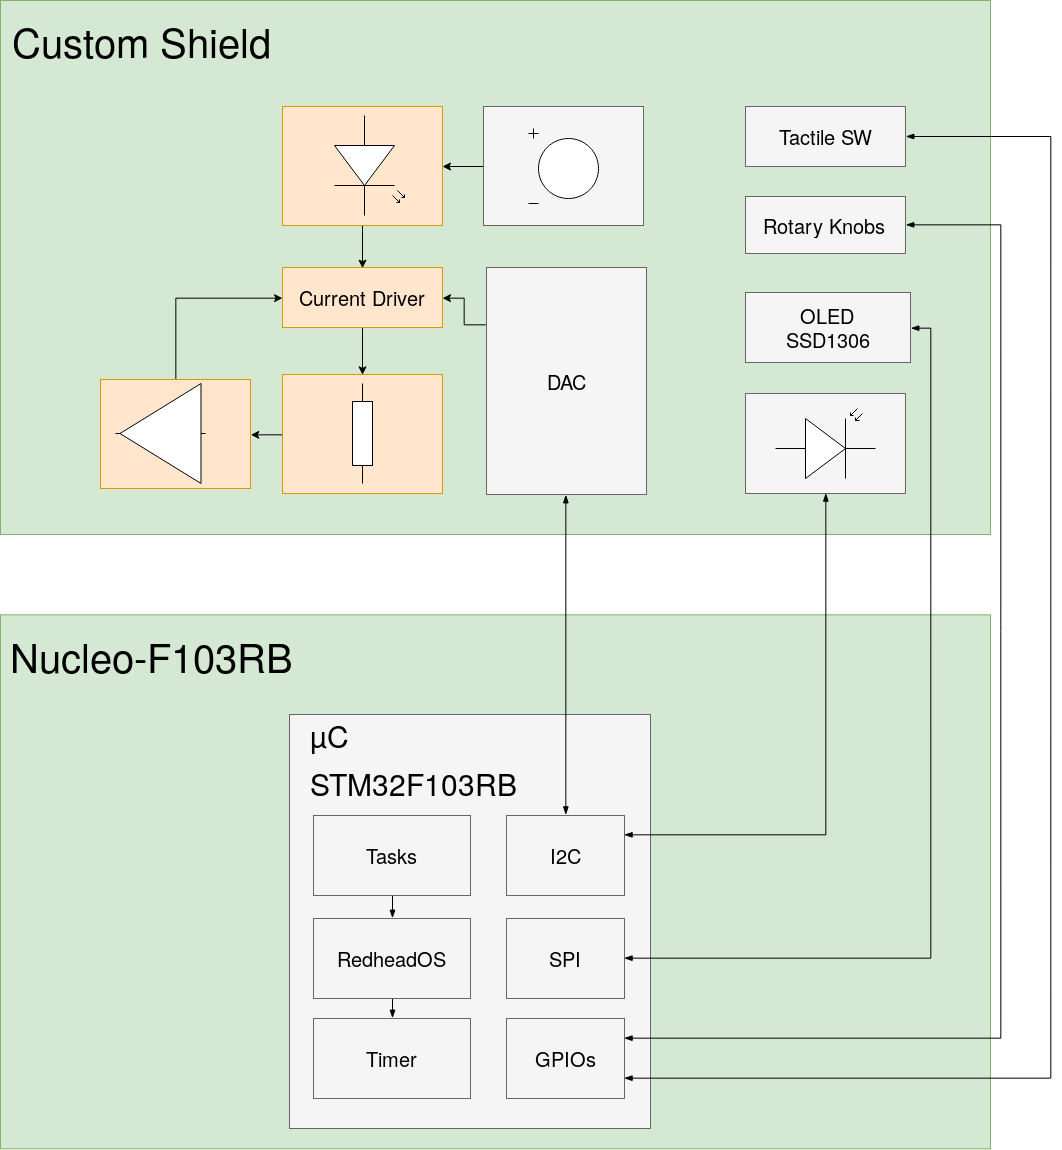
\includegraphics[scale=0.2]{./fig/uv_light}
 \end{figure}
 \end{frame}
 \section{State of the Art}
  	\begin{frame}{State of the Art}
		\begin{itemize}
			\item<1-> ARM-based 32 bit processor
			\item<2-> Self-designed current source
			\item<3-> SW-based controllers for aging effects compensation
			\item<4-> SW-based controllers for temperature regulation
		\end{itemize}
  	\end{frame}	
  \begin{frame}[standout]
	Happy Coding :) 
  \end{frame}
\end{document}
